\documentclass[a4paper,11pt,poets,durations]{ConcProg}
\renewcommand*\rmdefault{iwona}
\usepackage[utf8]{inputenc}
\usepackage[square,numbers]{natbib}
\usepackage[T1]{fontenc}
\usepackage{lmodern}
\usepackage{amsmath}
\usepackage{amssymb}
\usepackage{amsthm}
\usepackage{dsfont}
\usepackage{cancel}
\usepackage{graphicx}
\usepackage{geometry}
\usepackage[all]{xy}
\usepackage{graphicx}
\usepackage{microtype}
\usepackage[colorlinks=false, pdfborder={0 0 0}]{hyperref}
\setlength{\parindent}{0pt}

\begin{document}

{
\fontfamily{ppl}\selectfont

~\\

\begin{programme}{
    Concerts Trouvères @ Nuit 2016
\\  {\normalsize 26 novembre 2016, Pot-Actes-Beckett}
}
~\\
\begin{center}
\textsc{Buffet (20h15--21h00)}
\end{center}
  \begin{part}[]
    \begin{composition}{\dots}{}{Set de Jazz}{}
      {\small Jessica Joli (Chant) et [son guitariste]}
    \end{composition}\\
~\\
~\\
~\\
\begin{center}
\textsc{Valse (23h45--00h30)}
\end{center}
    \begin{composition}{Frédéric Chopin}{}{\dots}{\dots}
      {\small Timothée Bénard (Piano)}
    \end{composition}
    \begin{composition}{\dots}{}{\dots}{\dots}
      {\small Mehdi Trense (Piano)}
    \end{composition}
    \begin{composition}{Dmitri Chostakovitch}{}{Suite pour orchestre de variété no.1, op. 50b}{Valse no.2}
      {\small Anna Song (Piano), Timothée Bénard (Piano)}
    \end{composition}
    \begin{composition}{Johann Strauss II}{arr. Alban Berg}{Wein, Weib und Gesang, op. 333}{}
      {\small Gabriel Sulem (Violon), Benjamin David (Violon), Hugo Cui (Alto), Mylène Sauty (Violoncelle), Yichao Huang (Piano)}
    \end{composition}
    \begin{composition}{Johann Strauss II}{arr. Anton Webern}{Schatzwalzer, op. 418}{}
      {\small Gabriel Sulem (Violon), Benjamin David (Violon), Hugo Cui (Alto), Mylène Sauty (Violoncelle), Yichao Huang (Piano)}
    \end{composition}\\
~\\
~\\
~\\
\begin{center}
\textsc{Tango (00h15--01h00)}
\end{center}
    \begin{composition}{Aleksey Igudesman}{}{Go to tango town}{}
      {\small Déborah Sulem (Violon), Gabriel Sulem (Violon)}
    \end{composition}
    \begin{composition}{Aleksey Igudesman}{}{Tango sin nombre}{}
      {\small Déborah Sulem (Violon), Gabriel Sulem (Violon)}
    \end{composition}
    \begin{composition}{Astor Piazzolla}{arr. Vyacheslav Gryaznov}{Oblivion}{}
      {\small Gabriel Sulem (Violon), Benjamin David (Violon), Hugo Cui (Alto), Mylène Sauty (Violoncelle), Yichao Huang (Piano)}
    \end{composition}
    \begin{composition}{Karol Beffa}{}{Café 2010}{}
      {\small Gabriel Sulem (Violon), Benjamin David (Violon), Hugo Cui (Alto), Mylène Sauty (Violoncelle), Yichao Huang (Piano)}
    \end{composition}\\
~\\
~\\
~\\
\begin{center}
\textsc{Ordre de passage et minutages approximatifs.\\Les instruments seront stockés en salles [Cavaillès] et [Résistants].}\\
~\\
\begin{tabular}{rl}
\textsc{Yichao (Trouvère)} & \textsc{07 86 52 27 21 ;}\\
\textsc{Sarah (Buffet)} & \textsc{07 83 78 94 20 ;}\\
\textsc{Ludovic (Valse)} & \textsc{06 84 66 70 79 ;}\\
\textsc{Christophe (Tango)} & \textsc{07 81 90 10 39 ;}\\
\textsc{Apolline (Nuit)} & \textsc{06 45 34 27 42.}
\end{tabular}
\end{center}
  \end{part}
\end{programme}
}
\begin{center}
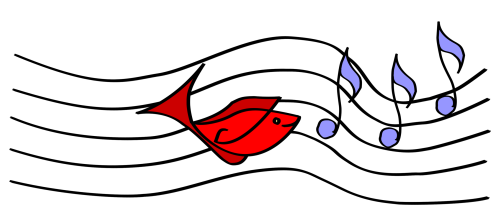
\includegraphics[scale=2]{logo.png}
\end{center}

\end{document}